%%%%%%%%%%%%%%%%%%%%%%%%%%%%%%%%%%%%%%%%%%%%%%%%%%%%%%%%%%%%%%%%%%%%%%%%%%%%
% AGUJournalTemplate.tex: this template file is for articles formatted with LaTeX
%
% This file includes commands and instructions
% given in the order necessary to produce a final output that will
% satisfy AGU requirements, including customized APA reference formatting.
%
% You may copy this file and give it your
% article name, and enter your text.
%
%
% Step 1: Set the \documentclass
%
%

%% To submit your paper:
\documentclass[draft]{agujournal2019}
\usepackage{url} %this package should fix any errors with URLs in refs.
\usepackage{lineno}
\usepackage[inline]{trackchanges} %for better track changes. finalnew option will compile document with changes incorporated.
\usepackage{soul}
\linenumbers
%%%%%%%
% As of 2018 we recommend use of the TrackChanges package to mark revisions.
% The trackchanges package adds five new LaTeX commands:
%
%  \note[editor]{The note}
%  \annote[editor]{Text to annotate}{The note}
%  \add[editor]{Text to add}
%  \remove[editor]{Text to remove}
%  \change[editor]{Text to remove}{Text to add}
%
% complete documentation is here: http://trackchanges.sourceforge.net/
%%%%%%%

\draftfalse

%% Enter journal name below.
%% Choose from this list of Journals:
%
% JGR: Atmospheres
% JGR: Biogeosciences
% JGR: Earth Surface
% JGR: Oceans
% JGR: Planets
% JGR: Solid Earth
% JGR: Space Physics
% Global Biogeochemical Cycles
% Geophysical Research Letters
% Paleoceanography and Paleoclimatology
% Radio Science
% Reviews of Geophysics
% Tectonics
% Space Weather
% Water Resources Research
% Geochemistry, Geophysics, Geosystems
% Journal of Advances in Modeling Earth Systems (JAMES)
% Earth's Future
% Earth and Space Science
% Geohealth
%
% ie, \journalname{Water Resources Research}

\journalname{Geophysical Research Letters}


\begin{document}

%% ------------------------------------------------------------------------ %%
%  Title
%
% (A title should be specific, informative, and brief. Use
% abbreviations only if they are defined in the abstract. Titles that
% start with general keywords then specific terms are optimized in
% searches)
%
%% ------------------------------------------------------------------------ %%

% Example: \title{This is a test title}

\title{Surface ocean warming around Australia driven by interannual variability and long-term trends in Southern Hemisphere westerlies}

%% ------------------------------------------------------------------------ %%
%
%  AUTHORS AND AFFILIATIONS
%
%% ------------------------------------------------------------------------ %%

% Authors are individuals who have significantly contributed to the
% research and preparation of the article. Group authors are allowed, if
% each author in the group is separately identified in an appendix.)

% List authors by first name or initial followed by last name and
% separated by commas. Use \affil{} to number affiliations, and
% \thanks{} for author notes.
% Additional author notes should be indicated with \thanks{} (for
% example, for current addresses).

% Example: \authors{A. B. Author\affil{1}\thanks{Current address, Antartica}, B. C. Author\affil{2,3}, and D. E.
% Author\affil{3,4}\thanks{Also funded by Monsanto.}}

\authors{E. R. Duran\affil{1,2}, M. H. England\affil{2,3}, and P.
Spence\affil{2,3}}


% \affiliation{1}{First Affiliation}
% \affiliation{2}{Second Affiliation}
% \affiliation{3}{Third Affiliation}
% \affiliation{4}{Fourth Affiliation}

\affiliation{1}{ARC Centre of Excellence for Climate System Science (ARCCSS), Sydney, NSW 2052 Australia}
\affiliation{2}{Climate Change Research Centre (CCRC), University of New South Wales, Sydney, NSW 2052 Australia}
\affiliation{3}{ARC Centre of Excellence for Climate Extremes (CLEX), Sydney, NSW 2052 Australia}
%(repeat as many times as is necessary)

%% Corresponding Author:
% Corresponding author mailing address and e-mail address:

% (include name and email addresses of the corresponding author.  More
% than one corresponding author is allowed in this LaTeX file and for
% publication; but only one corresponding author is allowed in our
% editorial system.)

% Example: \correspondingauthor{First and Last Name}{email@address.edu}

\correspondingauthor{E. R. Duran}{e.duran@student.unsw.edu.au}

%% Keypoints, final entry on title page.

%  List up to three key points (at least one is required)
%  Key Points summarize the main points and conclusions of the article
%  Each must be 100 characters or less with no special characters or punctuation and must be complete sentences

% Example:
% \begin{keypoints}
% \item	List up to three key points (at least one is required)
% \item	Key Points summarize the main points and conclusions of the article
% \item	Each must be 100 characters or less with no special characters or punctuation and must be complete sentences
% \end{keypoints}

\begin{keypoints}
\item Interannual southward shifts in Southern Hemisphere westerlies lead to surface ocean warming events in the South Australian Basin

\item CMIP5 $21^{st}$ Century projections suggest that wind trends will play a role comparable to global warming in driving surface ocean warming around Australia

\item $21^{st}$ Century wind trends are estimated to be responsible for around half of the projected surface ocean warming and sea level rise in the Tasman Sea
\end{keypoints}

%% ------------------------------------------------------------------------ %%
%
%  ABSTRACT and PLAIN LANGUAGE SUMMARY
%
% A good Abstract will begin with a short description of the problem
% being addressed, briefly describe the new data or analyses, then
% briefly states the main conclusion(s) and how they are supported and
% uncertainties.

% The Plain Language Summary should be written for a broad audience,
% including journalists and the science-interested public, that will not have 
% a background in your field.
%
% A Plain Language Summary is required in GRL, JGR: Planets, JGR: Biogeosciences,
% JGR: Oceans, G-Cubed, Reviews of Geophysics, and JAMES.
% see http://sharingscience.agu.org/creating-plain-language-summary/)
%
%% ------------------------------------------------------------------------ %%

%% \begin{abstract} starts the second page

\begin{abstract}
The ocean surface temperature and sea level response around Australia to both interannual variability as well as observed and projected changes in surface winds is presented. A hindcast ocean experiment shows interannual southward shifts in the Southern Hemisphere westerly winds drive ocean surface warming events in the South Australian Basin. Twenty-first Century climate and ocean projections in an ensemble of CMIP5 models show that wind trends will play a role comparable to global warming in driving surface ocean warming in this region. To evaluate the wind's role in these projected changes, we use an ocean experiment perturbed by the projected $21^{st}$ Century wind trends to show that the wind trends alone can generate approximately half of the ocean surface warming and sea level rise predicted by the CMIP5 models in the Tasman Sea.
\end{abstract}

\section*{Plain Language Summary}
The article demonstrates that both the year-to-year variability and the future projected trends in the Southern Hemisphere westerly winds are a major driver of surface ocean warming around Australia. Our research finds that year-to-year southward shifts in the Southern Hemisphere westerly winds lead to surface ocean warming events in the South Australian Basin. In future global warming projections, wind trends will also play a role comparable to global warming in driving surface ocean warming around Australia. To evaluate the wind's role in these projected changes, we apply the future projected winds to an ocean model experiment to show that, in the Tasman Sea, the wind trends alone can create about half of the surface ocean warming and half of the sea level rise predicted in the future global warming projections.


%% ------------------------------------------------------------------------ %%
%
%  TEXT
%
%% ------------------------------------------------------------------------ %%

%%% Suggested section heads:
% \section{Introduction}
%
% The main text should start with an introduction. Except for short
% manuscripts (such as comments and replies), the text should be divided
% into sections, each with its own heading.

% Headings should be sentence fragments and do not begin with a
% lowercase letter or number. Examples of good headings are:

% \section{Materials and Methods}
% Here is text on Materials and Methods.
%
% \subsection{A descriptive heading about methods}
% More about Methods.
%
% \section{Data} (Or section title might be a descriptive heading about data)
%
% \section{Results} (Or section title might be a descriptive heading about the
% results)
%
% \section{Conclusions}


\section{Introduction}
Future climate change is expected to drive oceanic surface warming on a global scale \cite{Stocker2013}. While some of this warming will be driven by radiative forcing effects, regimes of enhanced warming and cooling due to ocean circulation changes are also expected. For example, the $20^{th}$ Century poleward intensification (i.e. both an increase in strength and poleward shift in position) of western boundary currents was responsible for sea surface temperature (SST) increases two to three times higher over the western boundary currents than the global average \cite{Wu2012}. Indeed, one of the main ways global warming is altered in its signature in SST trends is due to wind-driven processes. For example, in the southern hemisphere, the seasonal poleward intensification of the westerly winds leads to surface cooling via increased upwelling of cooler subsurface water and strengthened northward transport \cite{Purich2016}. The southern hemisphere westerlies strength and meridional position is described by the Southern Annular Mode (SAM), which has been increasing since the 1950s \cite{Marshall2003}, with the westerlies shifting poleward and strengthening. The SAM is projected to further increase into the $21^{st}$ Century \cite{Gillett2013} and consequently drive ocean temperature changes due to changes in the mesoscale eddy field \cite{Screen2009}, Ekman pumping \cite{Purich2016}, and Southern Ocean fronts \cite{Spence2010}.

Here we present an Australian focus of the SST response to changes in the wind circulation associated with a positive SAM trend. Some previous studies have linked SST changes around Australia to the wind-driven circulation. For example, the East Australian Current (EAC) intensifies when the Pacific Ocean subtropical gyre shifts southward \cite{Hill2011}. A previous coupled-model global warming study showed that a SAM increase and an intensification of the EAC leads to to enhanced sea level rise and warming rates over the Tasman Sea \cite{Cai2005}. Another coupled-model experiment with a positive SAM trend showed a zonally symmetric SST warming between 30 $^{\circ}S$ and 50 $^{\circ}S$, encompassing the South Australian Basin, due to both a net surface heat flux gain via decreased wind-driven evaporative cooling and weaker northward advection of cold waters via decreased northward Ekman transport \cite{SenGupta2006}. While these experiments show a link between a positive SAM trend and warming in the Tasman Sea and in the South Australian Basin, the impact of interannual variability in the westerlies and the contribution of the winds alone to driving ocean surface warming around Australia has not yet been examined. In addition, there is no assessment to date of an ensemble of CMIP5 model projections for SST changes around Australia. This study will address these gaps in the literature.

In this work, we first use a hindcast experiment of an ocean model forced by an atmospheric reanalysis of the last 60 years to present the interannual variability of the winds and SST around Australia. Secondly, we diagnose projected $21^{st}$ Century regional climate change to test whether there is any association between projected SST changes and projected wind changes in the oceans around Australia. Finally, we perturb an ocean model using $21^{st}$ Century wind trends to test whether the wind projections alone, without any greenhouse gas radiative forcing changes, are sufficient to lead to changes in SST and oceanic processes around Australia. Our research underscores the importance of the Southern Hemisphere westerlies in shaping the subtropical latitude SST and sea level changes, both at interannual and long-term change time-scales, with these winds becoming increasingly significant as the SAM continues trending positive in a warming world.



\section{Methods}
\subsection{Hindcast experiment}
The past 60-years of SST, westerly winds and sea-level interannual variability in the South Australian Basin and the Tasman Sea is examined using a hindcast forced ocean model experiment. The model used is the Australian Community Climate and Earth-System Simulator (ACCESS-OM2-025, \citeA{Bi2012,Kiss2019}, \url{http://cosima.org.au/index.php/models/access-om2-025/}), run at a quarter degree resolution with 50 vertical levels and based on the Modular Ocean Model (MOM5.2, \citeA{Griffies2012}). In this hindcast experiment, ACCESS-OM2-025 is forced with an atmospheric reanalysis product configured for ocean model experiments (JRA-55 v1.3, \citeA{Kobayashi2015}, \url{http://jra.kishou.go.jp/JRA-55/index_en.html}), which spans the period 1958 to 2017. The model is run from initial conditions (World Ocean Atlas 2013, \citeA{Boyer2013}) with five cycles of JRA-55 atmospheric forcing; here we analyze the last 40 years (e.g. 1978-2017) of the final cycle.

\subsection{Twenty-first Century projections in CMIP5} \label{Twenty-first Century analysis in CMIP5}
Insight into the SST and sea-level response to $21^{st}$ Century climate change projections is determined from an analysis of the fifth phase of the Coupled Model Intercomparison Project (CMIP5, \citeA{Taylor2012}) models. The projections we consider here are under the RCP8.5 scenario, meaning that the rate of greenhouse gas emissions continues increasing through the $21^{st}$ Century, with no significant mitigation. All CMIP5 models show a positive SAM trend among these projections \cite{Bracegirdle2013}. However, this trend is zonally asymmetric across the models (not shown). In this work, we wish to examine the impact of poleward shifting winds over the southern Australia region, something that observational climatologies suggest is already underway \cite{Reichler2016}. Hence, to deal with the zonal asymmetry in the SAM trend, we only select those models that show a poleward wind shift south of Australia. To select these models we consider the 2080 to 2099 average zonal wind stress relative to the 1980 to 1999 average and ensure the zonal mean wind difference between $55\ ^{\circ}S$ and $36\ ^{\circ}S$ is positive in the vicinity of Australia (that is, over the range $100$--$140\ ^{\circ}E$, Fig.\ref{p25_fig2_}). This criterion is based on the zonal wind stress anomaly for each CMIP5 models with the latitudes selected to coincide with the location of westerlies weakening and westerlies strengthening, respectively. Only models with archived SST, zonal wind stress and wind speed components at 10 meters, both in the $21^{st}$ Century run and the historical run, are analysed; resulting in a total of 21 models for this analysis. We note that only 12 of the 21 models selected also include sea level height (see Fig.\ref{p25_fig2_}). We interpolate SST, zonal wind stress and sea level onto a common one degree grid and calculate the MMM wherever ocean grid points near land are included in at least half the models.

\subsection{Twenty-first Century winds experiment} \label{Twenty-first Century winds experiment}
To assess the wind contribution to driving SST changes around Australia, we devise two wind perturbation experiments using ACCESS-OM2-025 equilibrated with the CORE2-NYF atmospheric climatology (\citeA{Large2009},  \url{https://data1.gfdl.noaa.gov/nomads/forms/core/COREv2/CNYF_v2.html}). CORE2-NYF is ideal for running perturbation experiments as the prescribed atmospheric forcing does not include interannual variability and hence a statistical steady-state can be more readily reached. The model is first spun-up from initial conditions (World Ocean Atlas 2013, \citeA{Boyer2013}) with 500 years of CORE2-NYF. Next, a CMIP5 historical winds experiment is initialized with the CORE2-NYF spin-up and integrated for 70 years where the CORE2-NYF winds are replaced by the 1950 to 1969 averaged winds from the 21 CMIP5 models ensemble mean described in Section\,\ref{Twenty-first Century analysis in CMIP5}. Then, a $21^{st}$ Century winds experiment is initialized with this CMIP5 historical winds experiment and integrated for 70 years where the winds are replaced by the same CMIP5 ensemble mean but for the period 2080 to 2099. This experimental strategy is adopted because the CMIP5 models contain an equatorward wind bias \cite{Bracegirdle2013}; and so a comparison between a CMIP5-projected wind forced state and an observed forced simulation confounds the future trends with the present-day model biases. We instead analyse the CMIP5 $21^{st}$ Century winds experiment versus the CMIP5 historical winds experiment to obtain a more unambiguous ocean response to changes in the winds. Note that when we define the CMIP5 historical winds we select the 1950 to 1969 period as the baseline to capture the full SAM trend, which started increasing as early as the 1950s \cite{Marshall2003}. The implied southward shift in the westerlies and increase into the $21^{st}$ Century is depicted by zonal averages of zonal wind speed (Fig.\,\ref{p27_fig1_}a) and in the MMM zonal and meridional wind component anomalies (Fig.\,\ref{p27_fig1_}b,c). 

\section{Results and Discussion}
\subsection{Hindcast interannual variability experiment}
The trends and variability in annual mean zonal wind stress, SST and sea level during 1978 to 2017 in the JRA-55 hindcast experiment are examined in Fig.\,\ref{c08_fig1_}. The decadal trend in zonal wind stress (Fig.\,\ref{c08_fig1_}a) shows the westerly winds (located south of $30\ ^{\circ}S$) shifting southward, with a larger shift in the South Australian Basin than in the Tasman Sea. In the South Australian Basin, there is a corresponding weak SST increase (Fig.\,\ref{c08_fig1_}b,d) of $0.06\ \pm\ 0.03\ ^{\circ}C\ decade^{-1}$ (significant at $p$ = 0.03, Table\,\ref{Table3}) which could be due to decreased northward Ekman transport, since the westerly wind variability has a strong impact on the ocean circulation here \cite{Middleton2007}. In this region, the zonal wind stress strongly varies interannually (Fig.\,\ref{c08_fig1_}e) although there is no statistically significant long-term trend during 1978-2017 ($p$ = 0.40). Regardless, the linear regression between interannual variations in zonal wind stress and SST is significant ($R$ = -0.48 significant at $p$ $<$ 0.01), hence we examine composite anomalies of SST and zonal wind stress for the coldest and warmest SST years (Fig.\,\ref{c08_fig1_}d,e) to determine the westerly wind conditions during extreme SST years. In the South Australian Basin, we use a 0.9 standard deviation criterion to select the eight warmest SST years and we select the same amount of anomalous coldest SST years. Here, we find cold SST anomalies (Fig.\,\ref{c08_fig1_}h) when the westerlies are shifted northward (Fig.\,\ref{c08_fig1_}i) and warm SST anomalies (Fig.\,\ref{c08_fig1_}m) when the westerlies are shifted southward (Fig.\,\ref{c08_fig1_}l). This suggests that interannual shifts in the westerlies influence interannual variability in SST in this sector.

In the Tasman Sea, since warming of the ocean surface driven by the EAC strengthening is thought to be directly influenced by wind-driven circulation changes \cite{Hill2011,Oliver2014,Ridgway2007b,Roemmich2007,Wu2012}, we examine the relationship between sea level changes (a proxy for the gyre strength) and SST changes. Our results show a strong warming from 1978 to 2017 of $0.21\ \pm\ 0.04\ ^{\circ}C\ decade^{-1}$ (significant at $p$ $<$ 0.01) and a sea level rise of $2.2\ \pm\ 0.3\ cm\ decade^{-1}$ ($p$ $<$ 0.01, Table\,\ref{Table3}). Comparing over the shorter period with AVISO data availability, the 1993 to 2017 SST and sea level trends in the model (Fig.\,\ref{p01_c10}h,i,k,l) agree well with the same trends from satellite SST observations from NOOA OISST V2 (Fig.\,\ref{p01_c10}b,e) and satellite sea level overvations from AVISO (Fig.\,\ref{p01_c10}c,f). We find cold SST anomalies when sea level depresses (i.e. when the EAC flow weakens) and warm SST anomalies when sea level rises (i.e. when the EAC flow strengthens). Here, both SST and sea level trends are statistically significant ($p\ <\ 0.01$) and highly correlated ($R\ =\ 0.89$, Table\,\ref{Table3}). This Tasman Sea synchronous sea level rise with surface ocean warming was inferred previously \cite{Holbrook1997}, where past sea level rise events were correlated with wind stress curl intensification events east of New Zealand \cite{Roemmich2007}. However, sea level changes also come about due to local temperature changes via thermal expansion, so this correlation confounds EAC and gyre circulation changes with local temperature changes. It is thus of interest to further examine how much the sea level changes are driven by mechanical wind forcing versus due to thermal expansion. The $21^{st}$ Century wind experiment analysed in Section\,\ref{Twenty-first Century winds experiment} explores this question in more detail.

\begin{figure}[h]
\centering
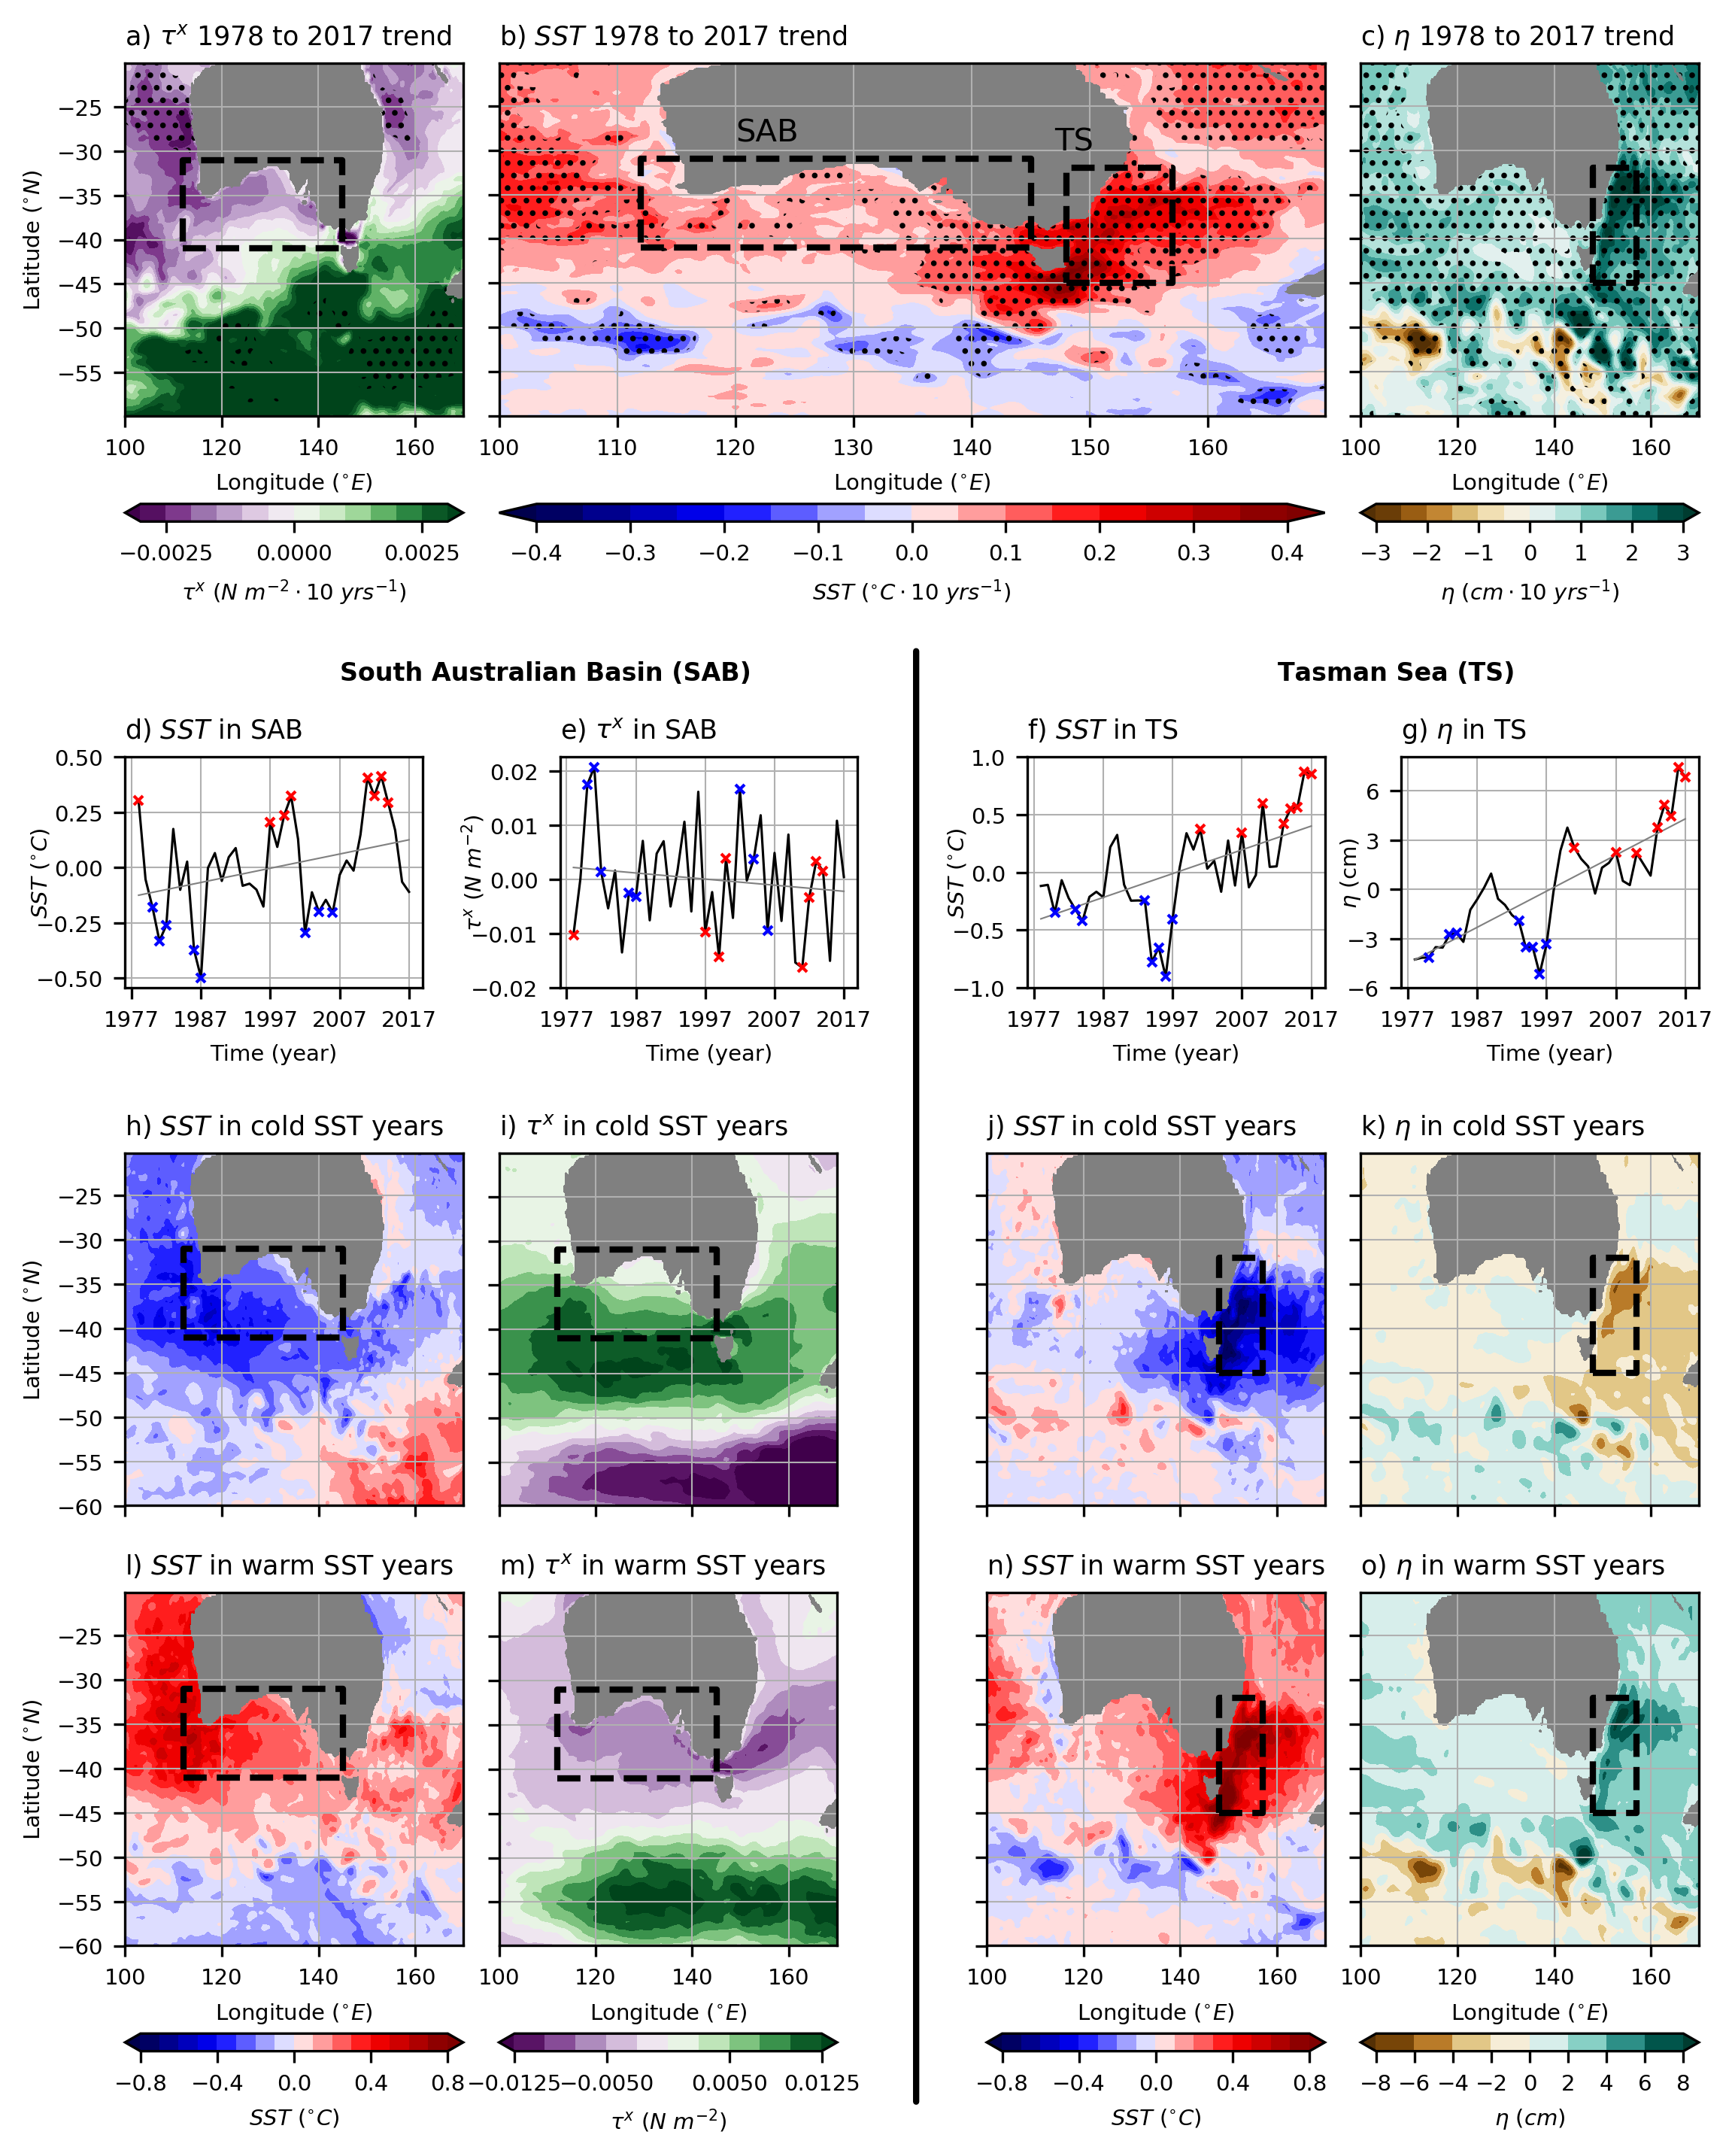
\includegraphics[trim={0 0.25cm 0 0},clip, width=1\textwidth]{c08_fig2_.png}
\caption{Results from the 1958-2017 experiment using ACCESS-OM2-025 forced by interannually varying forcing JRA-55 showing trends and variations in zonal wind stress ($N\ m^{-2}$), SST ($^{\circ}C$) and sea level ($cm$). Analyses are undertaken using annual-mean anomalies relative to the 1978 to 2017 mean. The top row shows the decadal trend estimated from the 1978 to 2017 linear trend. In the subsequent rows, SST and zonal wind stress are examined in the South Australian Basin area on the two left columns, and SST and sea level are examined in the Tasman Sea area on the two right columns. The second row shows the area averaged time series from 1978 to 2017 in (d,e) the South Australian Basin and (f,g) the Tasman Sea where blue (red) crosses point to the 8 years with coldest (warmest) area averaged SST. The third row shows the cold year composite average of (h,i) SST and zonal wind stress in the South Australian Basin and (j,k) SST and sea level in the Tasman Sea. The last row is the same as the above row, but for warm year composite averages.}\label{c08_fig1_}
\end{figure}


\subsection{Twenty-first Century CMIP5 projections}
We extend the analysis of zonal wind stress, ocean surface temperature and sea level variations into the $21^{st}$ Century using the RCP8.5 projections from the CMIP5 ensemble set. The following analyses compare the 2080 to 2099 average relative to the 1980 to 1999 average. Note that we have subsampled the CMIP5 ensemble to restrict to models that include a $21^{st}$ Century poleward wind shift in the Southern Australian region (Fig.\,\ref{p26_fig1_}a).

As a reminder, the RCP8.5 scenario means that the rate of greenhouse gas emissions continues increasing through the $21^{st}$ Century with no significant mitigation. Under this scenario, the MMM SST reveals a projected late $21^{st}$ Century ocean surface warming of up to $2.5\ ^{\circ}C$ in the South Australian Basin and up to $4.5\ ^{\circ}C$ in the Tasman Sea (Fig.\,\ref{p26_fig1_}b). In addition to warming, the MMM sea level increases everywhere including around Australia, particularly in the Tasman Sea, with up to $40\ cm$ projected sea level rise (Fig.\,\ref{p26_fig1_}c). Of course, we expect RCP8.5 MMM to show such a strong ocean thermal response because there is no significant greenhouse gas emission mitigation in this scenario, but we are also interested in how this varies across the simulations due to each model's different level of climate sensitivity. Here, climate sensitivity refers to the rate at which each model responds to climate change as measured by global average ocean surface temperatures. Our 21 model ensemble exhibits a large spread in this climate sensitivity metric across the models (Fig.\,\ref{p25_fig2_}).

We now explore the impact of this climate sensitivity spread in controlling southern Australian ocean warming relative to the key parameters in our two regions of interest, similar to the previous analysis in the JRA-55 hindcast experiment (i.e. SST versus zonal wind stress in the South Australian Basin and SST versus sea level in the Tasman Sea). In the South Australian Basin this model-by-model comparison reveals that models with the strongest poleward wind shift also tend to have the strongest ocean surface warming (Fig.\,\ref{p26_fig1_}d). This is because poleward shifting westerlies lead to a weakening of the wind belt over the South Australian Basin. The correlation between zonal wind stress and SST here shows the inter-model variability in SST can be well described by changes in the winds alone ($R^2$=0.74 significant at $p$ $<$ 0.001). Since the $21^{st}$ Century experiments are forced by increasing greenhouse gas emissions, part of the warming variation across models in the South Australian Basin could be due to each model's sensitivity to radiative forcing. This is examined by looking at the direct relationship between South Australian Basin SST and global SST (using the global SST trend as a proxy for radiative warming sensitivity, Fig.\,\ref{p26_fig1_}e). The inter-model correlation between local SST and global SST ($R^2$=0.58, $p$ $<$ 0.001) is significant, indicating climate sensitivity is also playing a key role here, but the correlation between local SST and zonal wind stress is even greater, suggesting that wind trends are at least as significant as global warming sensitivity in driving SST changes in this region.

In the Tasman Sea, models with the strongest sea level rise also tend to have the strongest ocean surface warming (Fig.\,\ref{p26_fig1_}f). Sea-level changes are due to both local ocean heat content changes, as well as circulation changes in the EAC. As above, the variability in local SST is better explained by local changes in sea level ($R^2$=0.76, $p$ $<$ 0.001) than by changes in global SST ($R^2$=0.63, $p$ $=$ 0.002, Fig.\,\ref{p26_fig1_}g), indicating that in this region, local ocean circulation changes are comparably significant to global warming model sensitivity in driving changes in SST. However, our analysis cannot separate out the effects of local radiative warming change from wind-stress forced gyre circulation and EAC changes, and so the exact contribution of the poleward wind shift in driving ocean surface warming is still unclear. In the next Section\,\ref{Twenty-first Century winds experiment} we use single-forced wind experiments to demonstrate that poleward intensifying winds are potentially going to be a dominant driver for surface ocean temperature changes around Australia over the $21^{st}$ Century.

\begin{figure}[h]
\centering
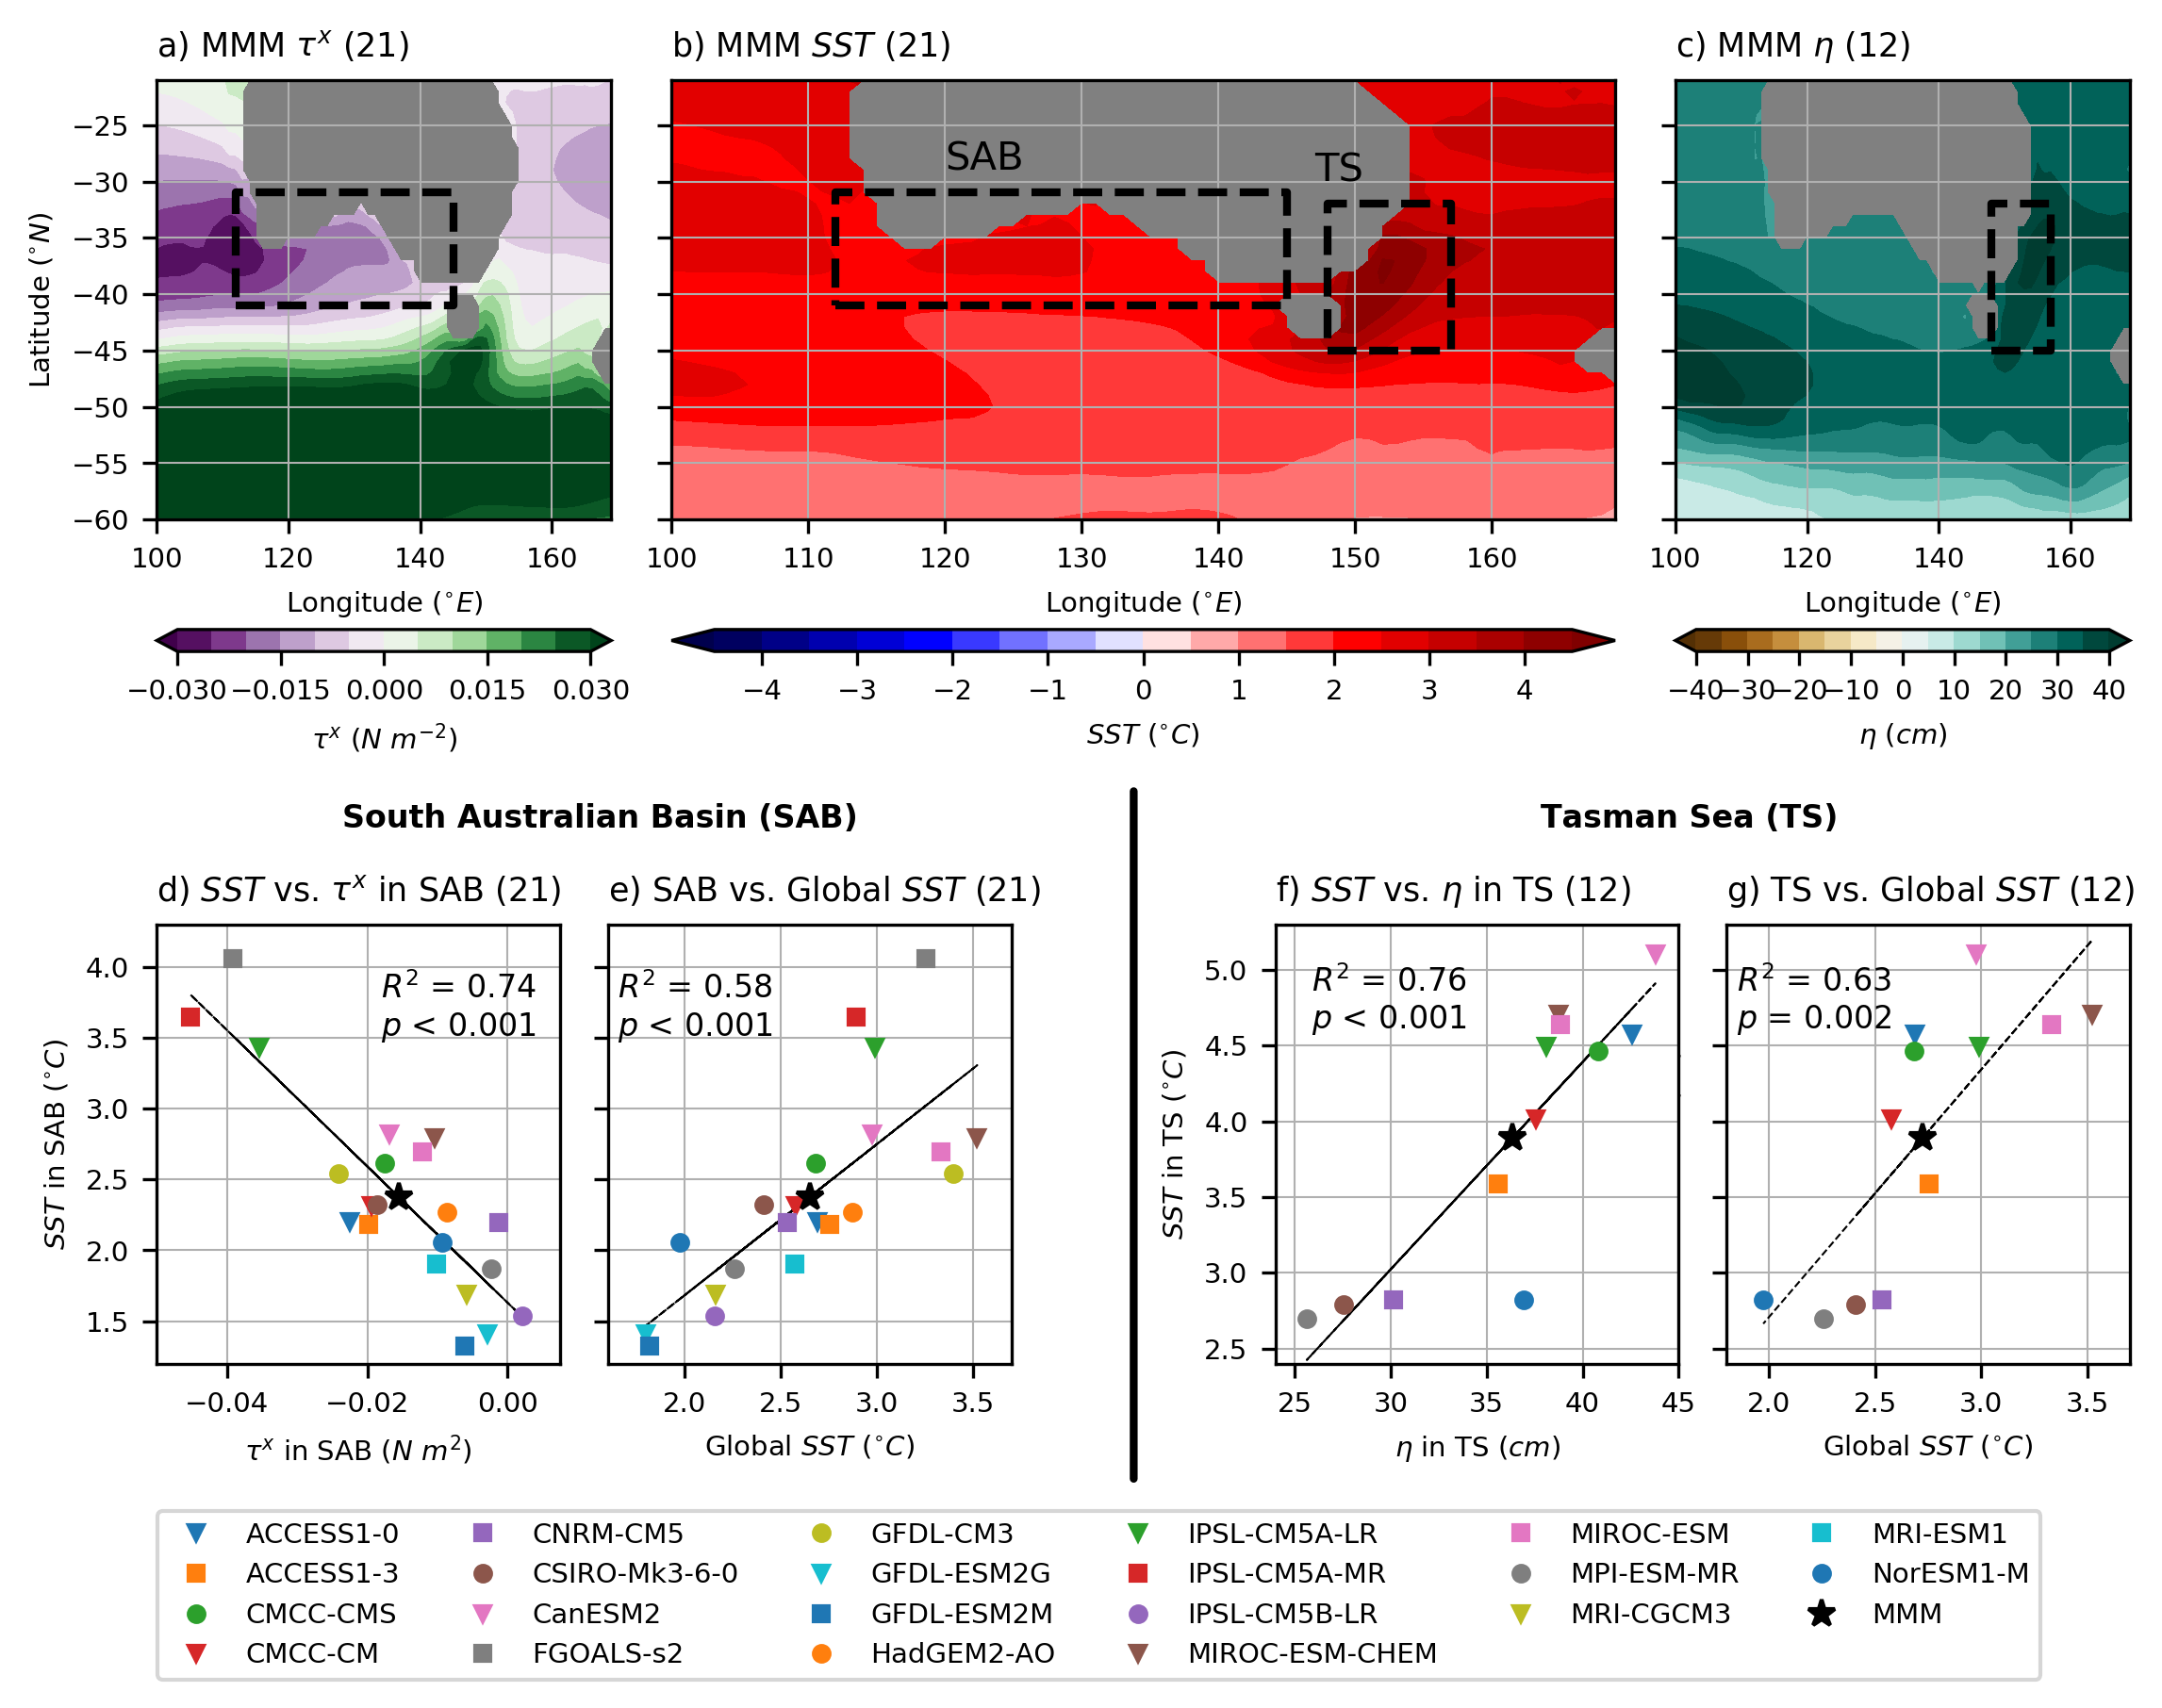
\includegraphics[trim={0 0 0 0},clip, width=1\textwidth]{p26_fig2_.png}
\caption{Analysis of twenty-one CMIP5 models exhibiting a positive SAM trend in the Australian sector showing zonal wind stress ($N\ m^{-2}$), SST ($^{\circ}C$) and sea level ($cm$). Properties are calculated as the 2080 to 2099 average relative to the 1980 to 1999 average. The top row shows the MMM from all models for zonal wind stress and SST and from twelve models for sea level (due to CMIP5 data availability). The bottom row left panels compare the area averaged SST in the South Australian Basin with (d) area averaged wind stress and (e) global mean SST (used as a proxy for climate sensitivity). The bottom row right panels compare the area averaged SST from available models in the Tasman Sea with (f) area averaged sea level and (g) global mean SST.}\label{p26_fig1_}
\end{figure}


\subsection{Twenty-first Century wind experiments} \label{Twenty-first Century winds experiment}
To isolate the contribution of the winds in driving SST changes, we now examine a $21^{st}$ Century wind perturbation experiment in ACCESS-OM2-025. First, a baseline historical CMIP5 winds experiment, initiated from a 500 years CORE2-NYF spin-up, is run for 70 years in which the CORE2-NYF winds are replaced by the 1950 to 1969 averaged winds from the 21 CMIP5 models ensemble mean described in the previous analysis. This is done to obtain a baseline experiment using CMIP5 historical winds to compare to the $21^{st}$ Century winds perturbation experiment. Then, the $21^{st}$ Century winds experiment is integrated for 70 years where the winds are replaced by the same 21 model CMIP5 ensemble mean but now averaged for the period 2080 to 2099. Note that because all other atmospheric fields are held fixed, particularly the air surface temperature, the SST response is actually damped back towards the historical CORE2-NYF forcing compared to what might be simulated in an unconstrained coupled model.

Fig.\,\ref{t09_fig1_} presents anomalies consisting of the final decadal average of the $21^{st}$ Century winds experiment relative to the historical 1950-1969 CMIP5 winds baseline experiment (see Fig.\,\ref{p27_fig1_}b,c for the corresponding wind anomaly). The SST anomaly (Fig.\,\ref{t09_fig1_}b) shows three distinctive patterns around Australia. Namely, there is a strong sea surface warming in the Tasman Sea that exceeds $2.25\ ^{\circ}C$ near southeast mainland Australia and Bass Strait. Sea surface cooling in contrast is found along the western and southern Australia continental shelves. Finally, over the oceans further south of Australia, the sea surface warms by up to $1.25\ ^{\circ}C$. At the same time, sea level is elevated in the Tasman Sea, particularly in the north around $32.5\ ^{\circ}S$, which is near the EAC separation region \cite{Godfrey1980}, and off the coast of southeast mainland Australia, with a sea level rise exceeding $20\ cm$ (Fig.\,\ref{t09_fig1_}c). Given the model experimental design, all these changes in SST and sea-level are entirely driven by winds and associated wind-driven changes in buoyancy fluxes.

These results demonstrate that the projected poleward intensified winds on their own are set to have a significant impact on SST and sea level around Australia. Remarkably, in the Tasman Sea, the contribution of the winds to sea surface warming ($2.25\ ^{\circ}C$) is about half of the warming simulated in the CMIP5 RCP8.5 projections analysed in the previous section ($4.5\ ^{\circ}C$, Fig.\,\ref{p26_fig1_}b). Similarly, the contribution of the winds to sea level rise in the Tasman Sea ($20\ cm$) is approximately half of the rise shown in the CMIP5 RCP8.5 projections ($40\ cm$, Fig.\,\ref{p26_fig1_}c). The magnitude of these SST changes is impressive given that fixed present-day seasonal atmospheric temperature fields were used to force the experiments, and that these act to damp the SST response toward present-day observations. This demonstrates the potential significant impact of projected wind-driven circulation changes as a driver of SST and sea level changes around Australia in the future.

To shed light on the mechanisms at play, additional properties are now also analysed. The anomalous net surface heat flux (Fig.\,\ref{t09_fig1_}e) shows that in the Tasman Sea, where a warming greater than $0.25\ ^{\circ}C$ occurs (thick contour lines), there is a corresponding net ocean heat loss from the ocean to the atmosphere. Here, the ocean heat loss pattern almost exactly matches the region of surface warming, confirming that wind driven circulation anomalies generate the surface warming and that atmospheric forcing then acts to damp it. In other words, ocean heat loss partially compensates for an excess heat gained via lateral ocean advection. This is consistent with \citeA{Cai2005}, who examined a series of global warming experiments to show ocean heat loss over the Tasman Sea coinciding with localised sea surface warming. 

The surface velocity field east of Australia (Fig.\,\ref{t09_fig1_}h) coincides with an increased transport in the south Pacific subtropical gyre (Fig.\,\ref{Bar_fig1_}c) and the EAC, which is consistent with \citeA{Hill2011}, who linked EAC strengthening to a southward shift in the Pacific Ocean gyre. The Tasman sea level anomaly (Fig.\,\ref{t09_fig1_}c) is linked, via geostrophy, with this anomalous gyre-like circulation. Here, the winds generate subtropical gyre and EAC spin up, leading to warming due to increased poleward heat transport in the EAC.

Along the coast of western and southern Australia, surface cooling occurs because of the slowdown of the warm southward flowing Leeuwin Current off western Australia (Fig.\,\ref{t09_fig1_}g) and its eastward extension along southern Australia (Fig.\,\ref{t09_fig1_}i). The slowdown is maintained by a weak coastal sea level drop (Fig.\,\ref{t09_fig1_}c) resulting in a pressure gradient working against the currents. The drop in sea-level is due to a reduction in eastward geostrophic flow toward the west Australian coast (Fig.\,\ref{Bar_fig1_}d), due to weakened westerly winds there (Fig.\,\ref{p27_fig1_}b). Furthermore, the wind stress curl (Fig.\,\ref{t09_fig1_}f) is largely negative off western and southern Australia, meaning that there is an anomalous upwelling flow along the shelf. Both the Leeuwin Current and the Southern Australia shelf break currents are downwelling-favourable currents along the shelf break \cite{Furue2017,Middleton2007}, due to strong onshore geostrophic flows off western Australia \cite{Godfrey1985} and onshore Ekman drift off southern Australia \cite{Middleton2007}. As a result, the atmosphere compensates for this advection-driven surface cooling via a heat gain across the air-sea interface (Fig.\,\ref{t09_fig1_}e). Hence, in contrast to the EAC strengthening, the poleward shift in the westerlies leads to a coastal sea level drop along southern and western Australia and a reduction of Ekman pumping which act to weaken the warm coastal currents.

Finally, in the ocean region further south of Australia, where a surface warming greater than $0.25\ ^{\circ}C$ occurs (Fig.\,\ref{t09_fig1_}b), there is a mix of net heat loss and heat gain from the ocean to the atmosphere (Fig.\,\ref{t09_fig1_}e). This implies that there are localised regions here where the ocean heat loss is compensating heat gained via ocean wind-driven advection, and other regions where the ocean warming is directly due to an anomalous heat gain from the atmosphere (due for example to anomalies in the wind-driven evaporative heat loss). To explain warming due to ocean lateral advection, changes in the meridional Ekman transport are presented (Fig.\,\ref{t09_fig1_}d) revealing the wind driven meridional transport in the Ekman layer derived from the applied wind perturbation. Weakening westerlies are associated with reduced northward Ekman transport of colder waters from the south \cite{SenGupta2006} as shown also in the broad southward surface flow anomaly in the western part of the South Australian Basin (Fig.\,\ref{Bar_fig1_}d, up to 3 $cm\ s^{-1}$ southward). Further south, in the Antarctic Circumpolar Current, strengthened westerlies have the opposite effect, leading to enhanced northward Ekman transport (Fig.\,\ref{t09_fig1_}d) and cooler ocean surface water there (Fig.\,\ref{t09_fig1_}b). To explain the warming due to ocean surface heat gain from the atmosphere, we note that the reduction of the winds there leads to a reduction in net evaporative heat loss at the ocean surface via reduced wind shear, and therefore a relative (anomalous) heat gain at the surface as also described in \citeA{SenGupta2006}. 

\begin{figure}[h]
\centering
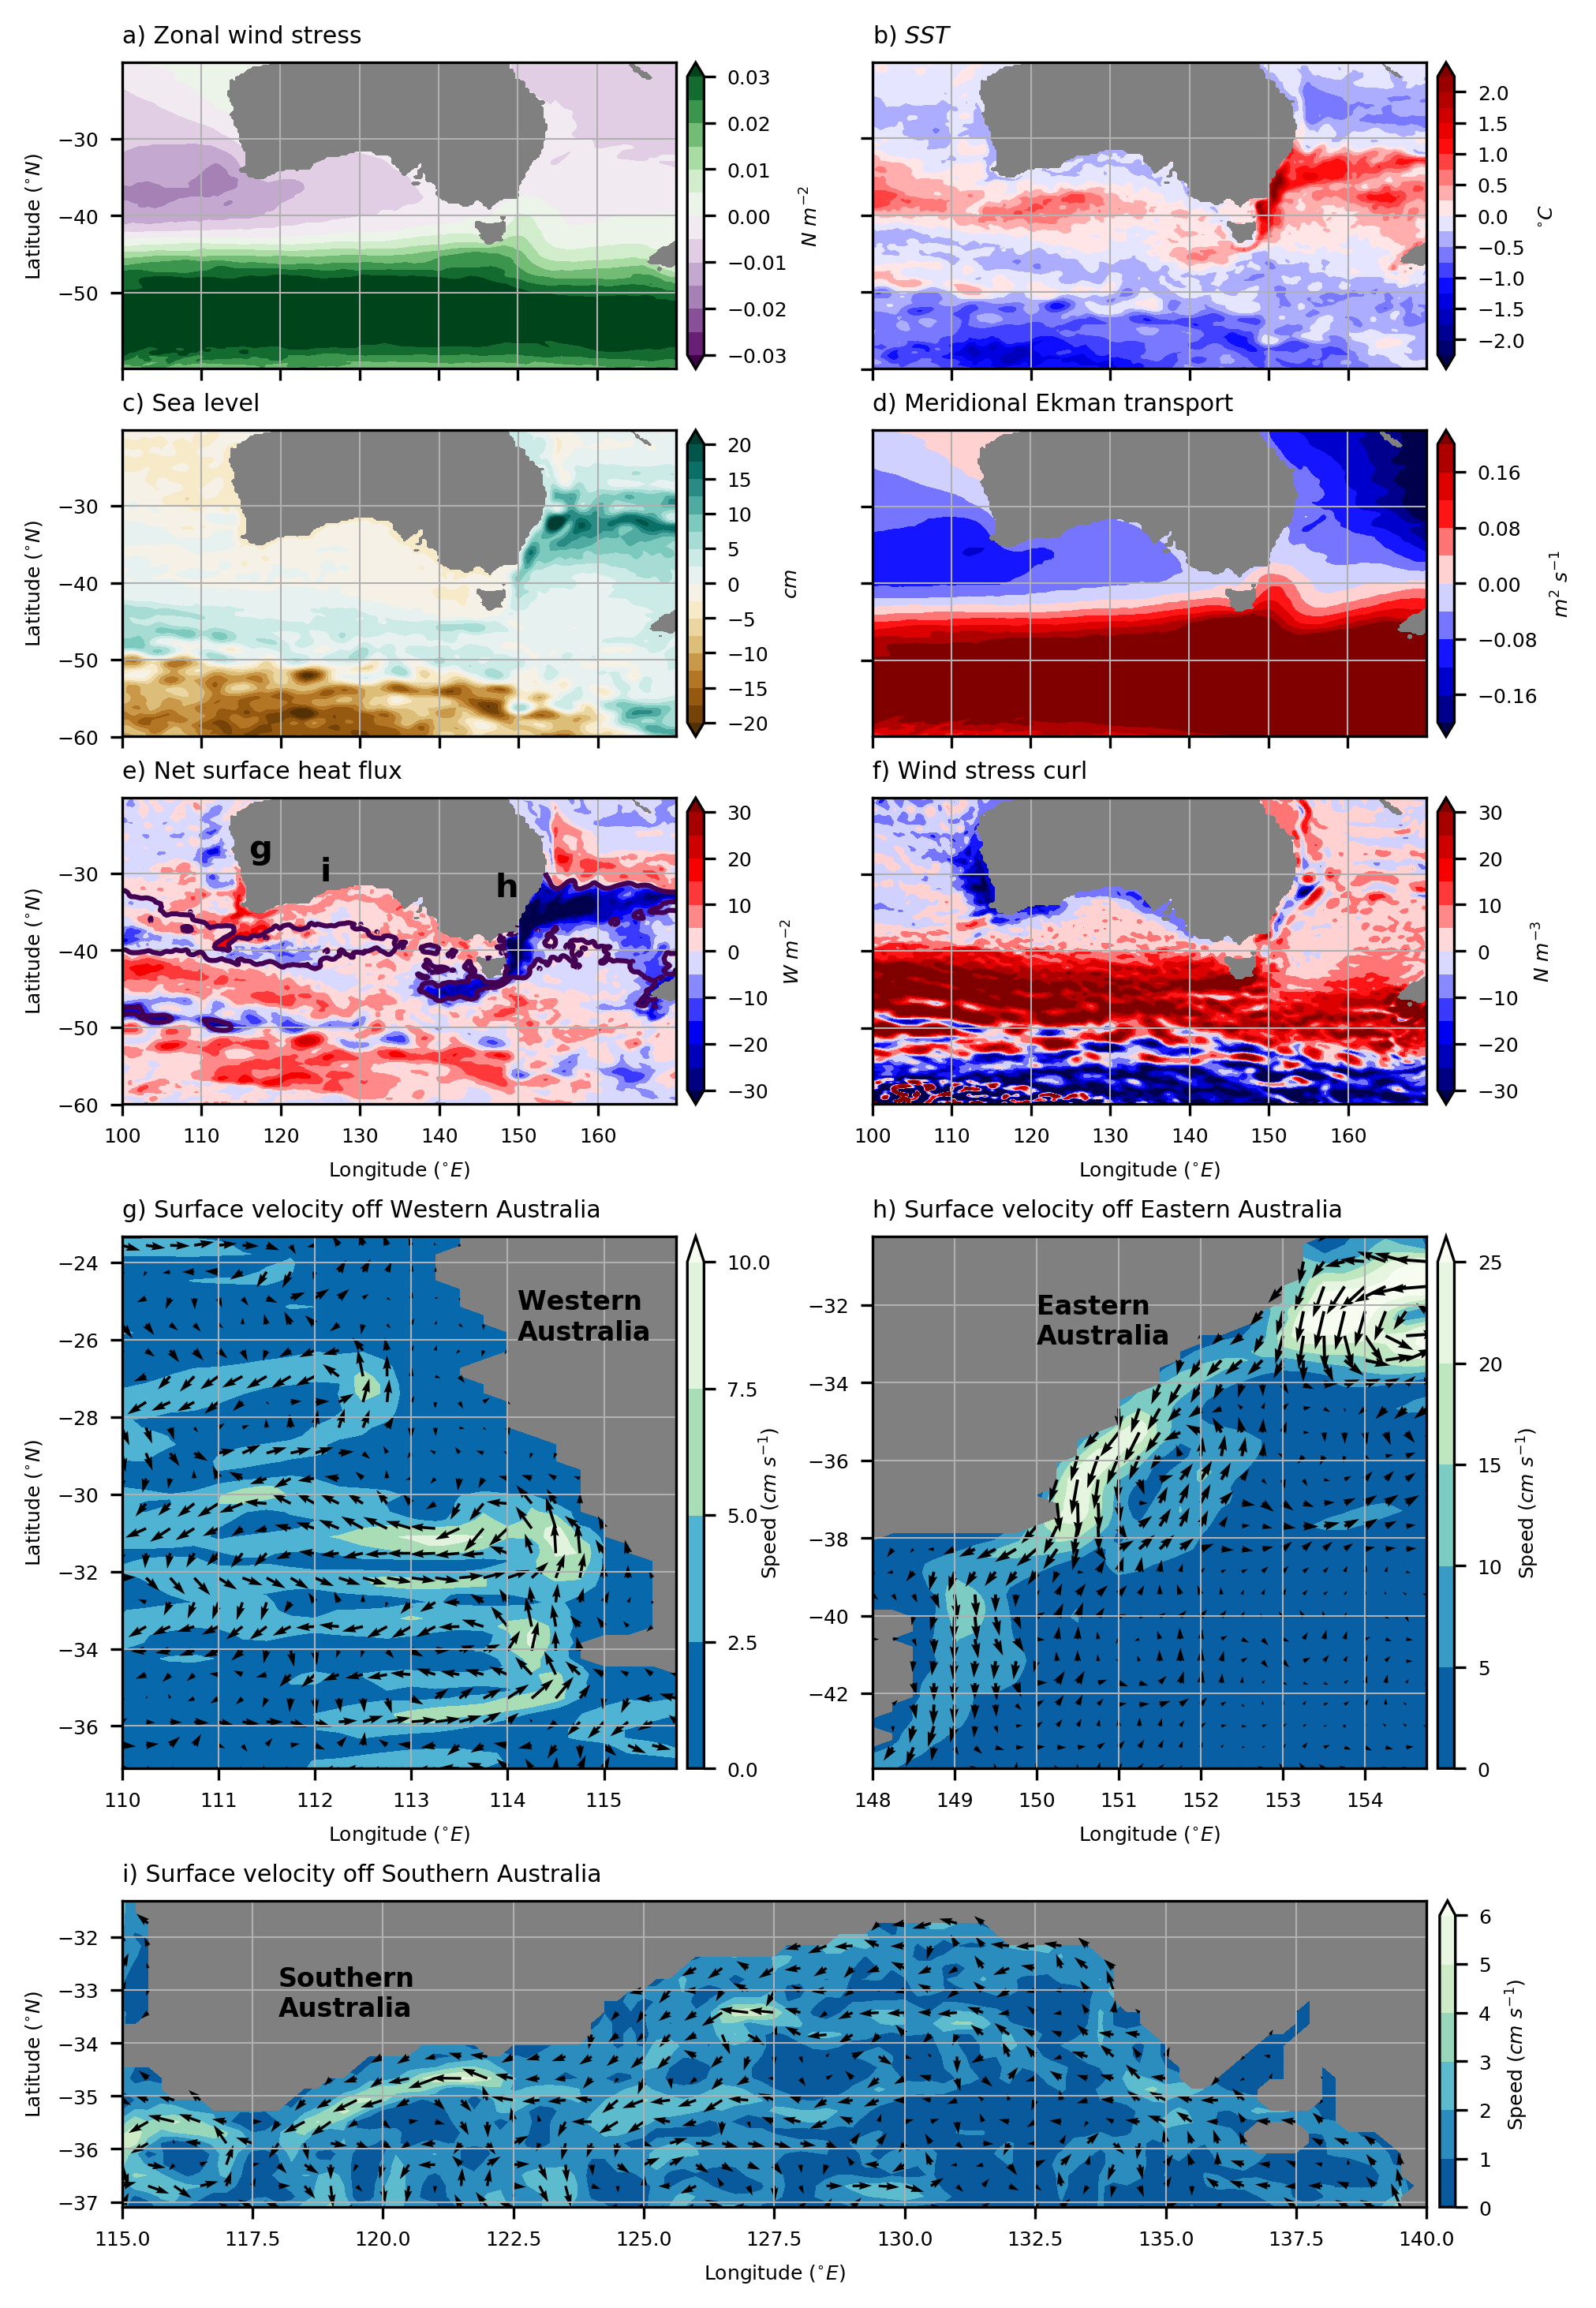
\includegraphics[trim={0 0.25cm 0cm 0.1cm},clip, width=0.98\textwidth]{t09_fig1_.png}
\caption{Results from the CMIP5 winds experiment using ACCESS-OM2-025 showing the last decadal average of the $21^{st}$ Century winds experiment relative to the CMIP5 historical winds experiment (see Section \ref{Twenty-first Century winds experiment} for experiments description). (a) Zonal wind stress ($N\ m^{-2}$), (b) SST ($^{\circ}C$), (c) sea level ($cm$), (d) meridional Ekman transport ($m^2\ s^{-1}$), (e) net surface heat flux ($W\ m^{-2}$), (f) wind stress curl ($N\ m^{-3}$) and surface velocity ($cm\ s^{-1}$) off (g) western Australia, (h) eastern Australia and (i) southern Australia. In (g-l), the arrows are proportional to the square root of the vector amplitudes to minimise the size of stronger flows. The solid contour lines in (e) enclose SST warming greater than $0.25\ ^{\circ}C$.}\label{t09_fig1_}
\end{figure}

\section{Summary and Conclusions}
A summary of the oceanic responses in the waters around Australia to wind anomalies associated with the projected positive SAM trend is presented in Fig.\,\ref{Slide1}. Our results show that, despite our experimental design resulting in damping of the SST response toward present-day surface temperature fields, the projected $21^{st}$ Century wind anomalies alone can drive significant ocean surface temperature changes, notably a warming in the Tasman Sea and in the region offshore of southern Australia, and a coastal cooling along the western and southern continental shelves. The wind-driven ocean surface warming in the Tasman Sea ($> 2.25 ^{\circ}C$), accounts for around half of the predicted warming in our analysis of the CMIP5 $21^{st}$ Century projections. The wind-driven warming is due to a stronger EAC driven by a spin-up of the subtropical gyre off eastern Australia, which produces enhanced poleward geostrophic flows (Fig.\,\ref{Slide1}). Elsewhere, the $21^{st}$ Century winds drive an alongshore cooling off western and southern Australia, as both the warm southward Leeuwin Current and the eastward flowing Southern Australia shelf break current are slowed down (Fig.\,\ref{Slide1}). Offshore of southern Australia, significant ocean surface warming occurs via reduced northward Ekman transport of cold waters from the south, as well as a reduction in net evaporative heat loss due to weaker wind speeds there (Fig.\,\ref{Slide1}).

In the South Australian Basin, results of the JRA-55 hindcast experiment also showed a strong SST sensitivity to interannual variability in westerly winds, where a southward shift in the westerlies can lead to significant ocean surface warming. This fast-time scale response is to be expected given the driving mechanism of surface Ekman flow alongside air-sea heat fluxes. The coupled model SAM increase response found in \citeA{SenGupta2006} showed a largely zonally symmetric southern hemisphere southward shift trend, which led to a corresponding band of warming where the westerlies weakened (approximately between $30$ and $50\ ^{\circ}S$). They found a conspiracy of elements leading to SST warming, namely, decreased heat loss to the atmosphere via decreased wind speeds, decreased northward advective cooling via decreased Ekman transport, and increased surface warming via increased sky clarity (i.e. less cloudy conditions). Here we suggest that, via the same mechanism, interannual southward shifts in the westerlies are an important driver of ocean surface temperature variability in the South Australian Basin. In our $21^{st}$ Century experiment, while an offshore warming is produced off eastern and southern Australia, the coastal cooling along the western and southern Australian shelves shows that the weakening of the mean local circulation acts against the broad warming induced by weakening westerlies in the South Australian Basin.

This work demonstrates that the westerly winds can play a major role in shaping both the interannual variability and long term trends in the Australian SST response to climate variability and climate change. This control of the winds over regional Australian SST is set to continue as increasing greenhouse gases drive further changes in the Southern Annular Mode. Given the severe ecological consequences of recently observed marine heatwaves around Australia (e.g. \citeA{Feng2013,Oliver2017}), this study suggests that monitoring changes in the wind-driven circulation around and south of Australia is critical to help understand and interpret future marine environmental changes.

\begin{figure}[h]
\centering
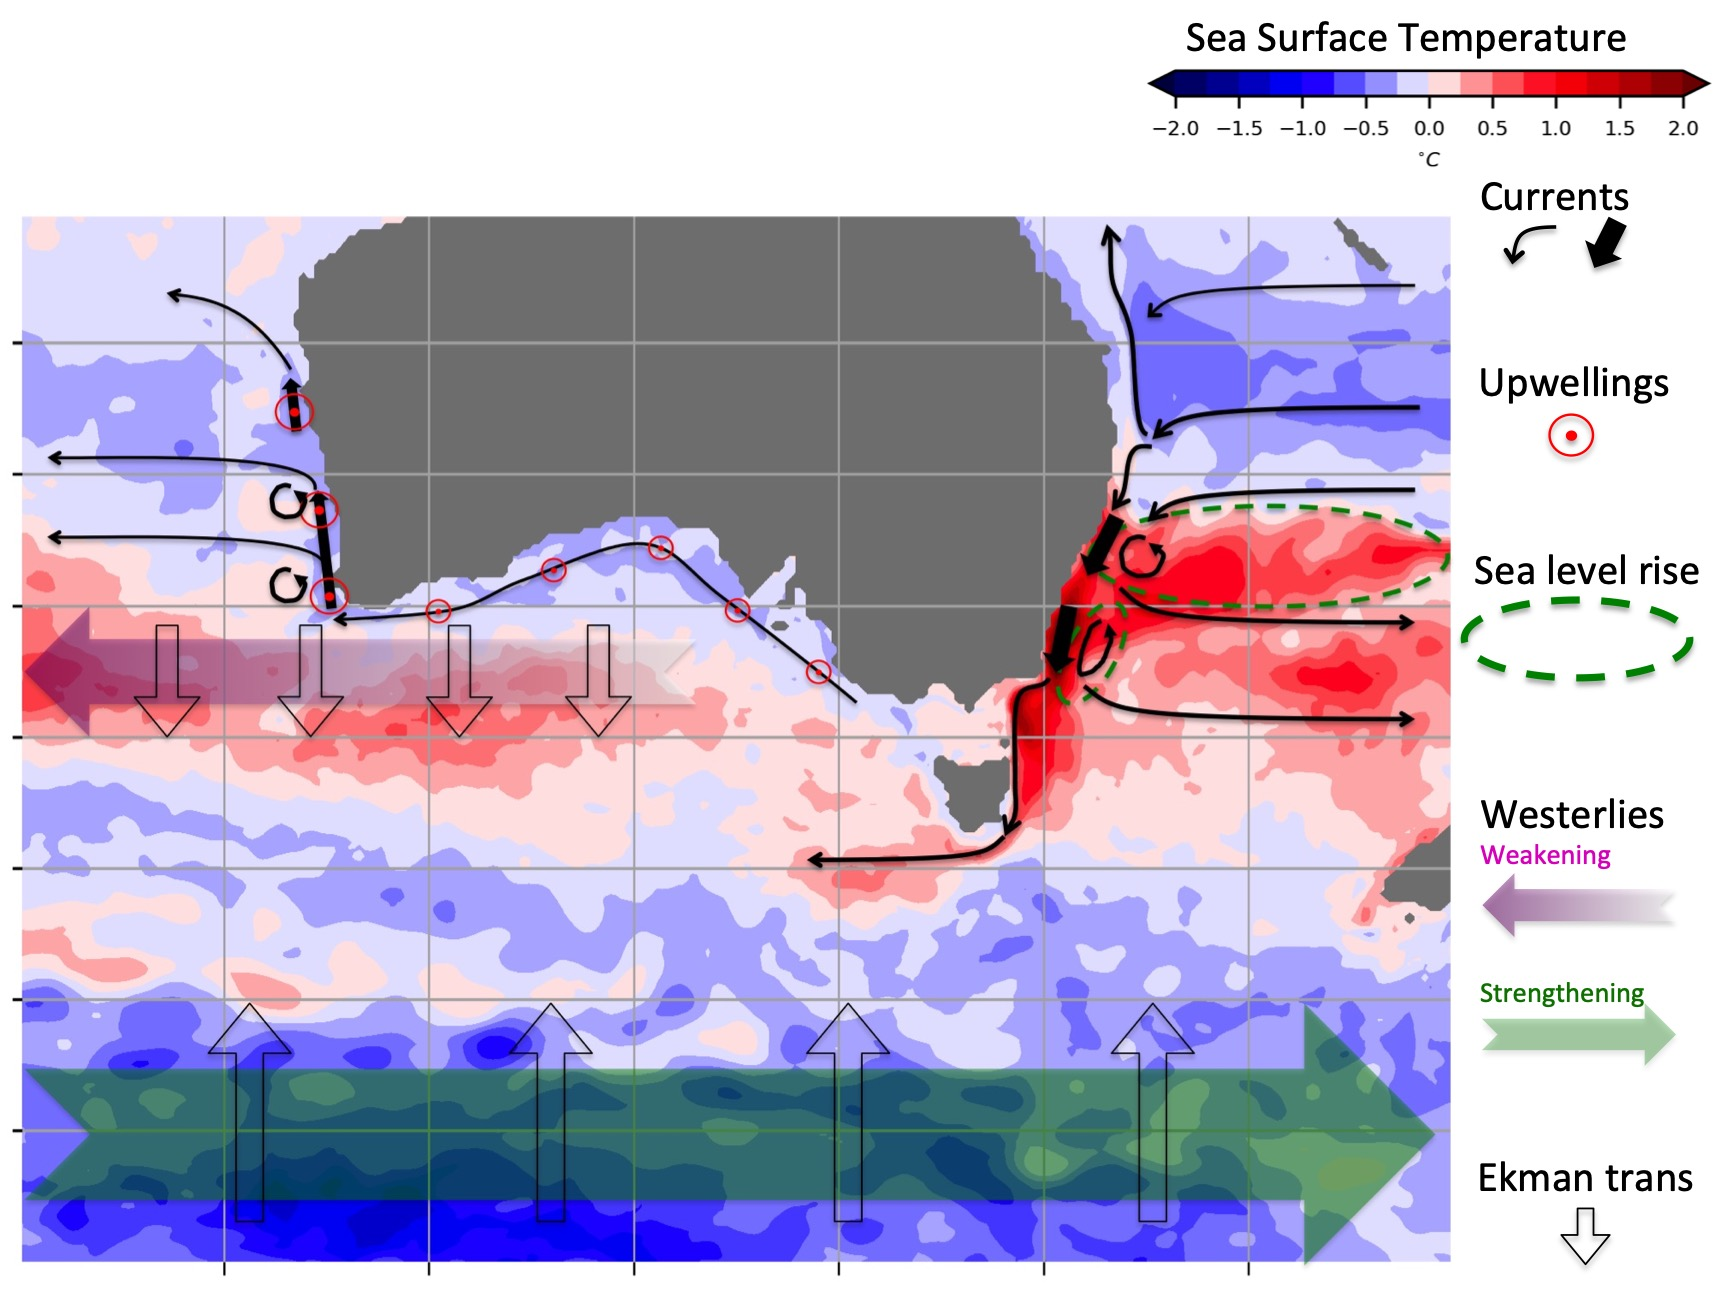
\includegraphics[width=1\textwidth]{Slide1.jpg}
\caption{Schematic summary of the response of the ocean to the $21^{st}$ Century wind perturbation. All properties are anomalies showing results from the $21^{st}$ Century CMIP5 winds experiment relative to the historical CMIP5 winds experiment. The background shading is the SST ($^{\circ}C$) anomaly. The Tasman Sea warming is due to a spin up of the anti-clockwise gyre circulation in the Tasman Sea. This circulation enhances the EAC which drives the strongest warming near the shelf. Offshore of southern Australia, the poleward intensified winds result in weaker northward Ekman transport immediately south of Australia where the westerlies weaken, and thus a warming anomaly there. Further south, enhanced westerlies drive stronger northward Ekman transport of cold fresh subantarctic surface water, cooling SST there. Along the western and southern Australian shelves, the downwelling Leeuwin Current and Southern Australia shelf break currents weaken and drive an alongshore cooling anomaly.}\label{Slide1}
\end{figure}


%Text here ===>>>


%%

%  Numbered lines in equations:
%  To add line numbers to lines in equations,
%  \begin{linenomath*}
%  \begin{equation}
%  \end{equation}
%  \end{linenomath*}



%% Enter Figures and Tables near as possible to where they are first mentioned:
%
% DO NOT USE \psfrag or \subfigure commands.
%
% Figure captions go below the figure.
% Table titles go above tables;  other caption information
%  should be placed in last line of the table, using
% \multicolumn2l{$^a$ This is a table note.}
%
%----------------
% EXAMPLE FIGURES
%
% \begin{figure}
% \includegraphics{example.png}
% \caption{caption}
% \end{figure}
%
% Giving latex a width will help it to scale the figure properly. A simple trick is to use \textwidth. Try this if large figures run off the side of the page.
% \begin{figure}
% \noindent\includegraphics[width=\textwidth]{anothersample.png}
%\caption{caption}
%\label{pngfiguresample}
%\end{figure}
%
%
% If you get an error about an unknown bounding box, try specifying the width and height of the figure with the natwidth and natheight options. This is common when trying to add a PDF figure without pdflatex.
% \begin{figure}
% \noindent\includegraphics[natwidth=800px,natheight=600px]{samplefigure.pdf}
%\caption{caption}
%\label{pdffiguresample}
%\end{figure}
%
%
% PDFLatex does not seem to be able to process EPS figures. You may want to try the epstopdf package.
%

%
% ---------------
% EXAMPLE TABLE
%
% \begin{table}
% \caption{Time of the Transition Between Phase 1 and Phase 2$^{a}$}
% \centering
% \begin{tabular}{l c}
% \hline
%  Run  & Time (min)  \\
% \hline
%   $l1$  & 260   \\
%   $l2$  & 300   \\
%   $l3$  & 340   \\
%   $h1$  & 270   \\
%   $h2$  & 250   \\
%   $h3$  & 380   \\
%   $r1$  & 370   \\
%   $r2$  & 390   \\
% \hline
% \multicolumn{2}{l}{$^{a}$Footnote text here.}
% \end{tabular}
% \end{table}

%% SIDEWAYS FIGURE and TABLE
% AGU prefers the use of {sidewaystable} over {landscapetable} as it causes fewer problems.
%
% \begin{sidewaysfigure}
% \includegraphics[width=20pc]{figsamp}
% \caption{caption here}
% \label{newfig}
% \end{sidewaysfigure}
%
%  \begin{sidewaystable}
%  \caption{Caption here}
% \label{tab:signif_gap_clos}
%  \begin{tabular}{ccc}
% one&two&three\\
% four&five&six
%  \end{tabular}
%  \end{sidewaystable}

%% If using numbered lines, please surround equations with \begin{linenomath*}...\end{linenomath*}
%\begin{linenomath*}
%\begin{equation}
%y|{f} \sim g(m, \sigma),
%\end{equation}
%\end{linenomath*}

%%% End of body of article

%%%%%%%%%%%%%%%%%%%%%%%%%%%%%%%%
%% Optional Appendix goes here
%
% The \appendix command resets counters and redefines section heads
%
% After typing \appendix
%
%\section{Here Is Appendix Title}
% will show
% A: Here Is Appendix Title
%
%\appendix
%\section{Here is a sample appendix}

%%%%%%%%%%%%%%%%%%%%%%%%%%%%%%%%%%%%%%%%%%%%%%%%%%%%%%%%%%%%%%%%
%
% Optional Glossary, Notation or Acronym section goes here:
%
%%%%%%%%%%%%%%
% Glossary is only allowed in Reviews of Geophysics
%  \begin{glossary}
%  \term{Term}
%   Term Definition here
%  \term{Term}
%   Term Definition here
%  \term{Term}
%   Term Definition here
%  \end{glossary}

%
%%%%%%%%%%%%%%
% Acronyms
%   \begin{acronyms}
%   \acro{Acronym}
%   Definition here
%   \acro{EMOS}
%   Ensemble model output statistics
%   \acro{ECMWF}
%   Centre for Medium-Range Weather Forecasts
%   \end{acronyms}

%
%%%%%%%%%%%%%%
% Notation
%   \begin{notation}
%   \notation{$a+b$} Notation Definition here
%   \notation{$e=mc^2$}
%   Equation in German-born physicist Albert Einstein's theory of special
%  relativity that showed that the increased relativistic mass ($m$) of a
%  body comes from the energy of motion of the body—that is, its kinetic
%  energy ($E$)—divided by the speed of light squared ($c^2$).
%   \end{notation}




%%%%%%%%%%%%%%%%%%%%%%%%%%%%%%%%%%%%%%%%%%%%%%%%%%%%%%%%%%%%%%%%
%
%  ACKNOWLEDGMENTS
%
% The acknowledgments must list:
%
% >>>>	A statement that indicates to the reader where the data
% 	supporting the conclusions can be obtained (for example, in the
% 	references, tables, supporting information, and other databases).
%
% 	All funding sources related to this work from all authors
%
% 	Any real or perceived financial conflicts of interests for any
%	author
%
% 	Other affiliations for any author that may be perceived as
% 	having a conflict of interest with respect to the results of this
% 	paper.
%
%
% It is also the appropriate place to thank colleagues and other contributors.
% AGU does not normally allow dedications.


\acknowledgments
Enter acknowledgments, including your data availability statement, here.


%% ------------------------------------------------------------------------ %%
%% References and Citations

%%%%%%%%%%%%%%%%%%%%%%%%%%%%%%%%%%%%%%%%%%%%%%%
%
% \bibliography{<name of your .bib file>} don't specify the file extension
%
% don't specify bibliographystyle
%%%%%%%%%%%%%%%%%%%%%%%%%%%%%%%%%%%%%%%%%%%%%%%

\bibliography{references.bib}



%Reference citation instructions and examples:
%
% Please use ONLY \cite and \citeA for reference citations.
% \cite for parenthetical references
% ...as shown in recent studies (Simpson et al., 2019)
% \citeA for in-text citations
% ...Simpson et al. (2019) have shown...
%
%
%...as shown by \citeA{jskilby}.
%...as shown by \citeA{lewin76}, \citeA{carson86}, \citeA{bartoldy02}, and \citeA{rinaldi03}.
%...has been shown \cite{jskilbye}.
%...has been shown \cite{lewin76,carson86,bartoldy02,rinaldi03}.
%... \cite <i.e.>[]{lewin76,carson86,bartoldy02,rinaldi03}.
%...has been shown by \cite <e.g.,>[and others]{lewin76}.
%
% apacite uses < > for prenotes and [ ] for postnotes
% DO NOT use other cite commands (e.g., \citeA, \cite, \citeyear, \nocite, \citeA, etc.).
%



\end{document}



More Information and Advice:

%% ------------------------------------------------------------------------ %%
%
%  SECTION HEADS
%
%% ------------------------------------------------------------------------ %%

% Capitalize the first letter of each word (except for
% prepositions, conjunctions, and articles that are
% three or fewer letters).

% AGU follows standard outline style; therefore, there cannot be a section 1 without
% a section 2, or a section 2.3.1 without a section 2.3.2.
% Please make sure your section numbers are balanced.
% ---------------
% Level 1 head
%
% Use the \section{} command to identify level 1 heads;
% type the appropriate head wording between the curly
% brackets, as shown below.
%
%An example:
%\section{Level 1 Head: Introduction}
%
% ---------------
% Level 2 head
%
% Use the \subsection{} command to identify level 2 heads.
%An example:
%\subsection{Level 2 Head}
%
% ---------------
% Level 3 head
%
% Use the \subsubsection{} command to identify level 3 heads
%An example:
%\subsubsection{Level 3 Head}
%
%---------------
% Level 4 head
%
% Use the \subsubsubsection{} command to identify level 3 heads
% An example:
%\subsubsubsection{Level 4 Head} An example.
%
%% ------------------------------------------------------------------------ %%
%
%  IN-TEXT LISTS
%
%% ------------------------------------------------------------------------ %%
%
% Do not use bulleted lists; enumerated lists are okay.
% \begin{enumerate}
% \item
% \item
% \item
% \end{enumerate}
%
%% ------------------------------------------------------------------------ %%
%
%  EQUATIONS
%
%% ------------------------------------------------------------------------ %%

% Single-line equations are centered.
% Equation arrays will appear left-aligned.

Math coded inside display math mode \[ ...\]
 will not be numbered, e.g.,:
 \[ x^2=y^2 + z^2\]

 Math coded inside \begin{equation} and \end{equation} will
 be automatically numbered, e.g.,:
 \begin{equation}
 x^2=y^2 + z^2
 \end{equation}


% To create multiline equations, use the
% \begin{eqnarray} and \end{eqnarray} environment
% as demonstrated below.
\begin{eqnarray}
  x_{1} & = & (x - x_{0}) \cos \Theta \nonumber \\
        && + (y - y_{0}) \sin \Theta  \nonumber \\
  y_{1} & = & -(x - x_{0}) \sin \Theta \nonumber \\
        && + (y - y_{0}) \cos \Theta.
\end{eqnarray}

%If you don't want an equation number, use the star form:
%\begin{eqnarray*}...\end{eqnarray*}

% Break each line at a sign of operation
% (+, -, etc.) if possible, with the sign of operation
% on the new line.

% Indent second and subsequent lines to align with
% the first character following the equal sign on the
% first line.

% Use an \hspace{} command to insert horizontal space
% into your equation if necessary. Place an appropriate
% unit of measure between the curly braces, e.g.
% \hspace{1in}; you may have to experiment to achieve
% the correct amount of space.


%% ------------------------------------------------------------------------ %%
%
%  EQUATION NUMBERING: COUNTER
%
%% ------------------------------------------------------------------------ %%

% You may change equation numbering by resetting
% the equation counter or by explicitly numbering
% an equation.

% To explicitly number an equation, type \eqnum{}
% (with the desired number between the brackets)
% after the \begin{equation} or \begin{eqnarray}
% command.  The \eqnum{} command will affect only
% the equation it appears with; LaTeX will number
% any equations appearing later in the manuscript
% according to the equation counter.
%

% If you have a multiline equation that needs only
% one equation number, use a \nonumber command in
% front of the double backslashes (\\) as shown in
% the multiline equation above.

% If you are using line numbers, remember to surround
% equations with \begin{linenomath*}...\end{linenomath*}

%  To add line numbers to lines in equations:
%  \begin{linenomath*}
%  \begin{equation}
%  \end{equation}
%  \end{linenomath*}



